\subsection{Cross validation}

Prima di introdurre la Cross Validation, o convalida incrociata, ci tengo a spiegare l'overfitting e l'underfitting.
\newline L'overfitting avviene quando il modello si trova in una condizione di sovradattamento, ovvero quando esso diventa troppo complesso e specifico per i dati di training che sta processando. Questo sovradattamento alle caratteristiche dei dati del training, porta il modello a non prevedere nuovi dati, avendo dunque risultati performanti in caso di training e risultati scarsi in caso di test. Si parla dunque di alta varianza, ovvero si presta troppa attenzione sui dati di training.
\newline L'underfitting invece avviene quando il modello non riesce ad approssimare bene i dati di training e quindi risulta inadatto anche ai dati di test. In questo caso si parla di alto bias e modello troppo semplice. 
\newline Per trovare il giusto compromesso, si effettua quella che viene chiamata \textbf{cross validation}. Questa tecnica ci permette di scegliere gli iperparametri ottimali del modello ("model selection").
Esistono diverse tecniche di cross validation, tra cui:
\begin{itemize}
    \item \textbf{Holdout}: Una porzione del training set viene splittata una tantum tra i dati di addestramento e quelli per valutarne le prestazioni, appunto, il validation set. Ciò però può determinare basse o alte prestazioni poichè dipende da quali samples sono finiti nel training e nel validation set
    \item \textbf{K-Fold}: Il training set viene diviso in k parti, dette fold, in cui k-1 vengono usate come trining e la restante come validation. Iterando k volte, cambiando ad ogni step quale porzione venga utilizzata come validation set, si ottengono delle prestazioni con cui si effettua la media sui k run.
    \item \textbf{Leave-One-Out}: il training set viene diviso in n-1 samples, il validation con solo un sample. Ripetendo n volte, si ottiene lo scoring come media delle n prestazioni sugli n run.
\end{itemize}
Esiste poi la "Stratificazione", ovvero si fa in modo (che si usi KFold o Holdout) di avere \textbf{proporzionalmente} il numero di sample di ciascuna classe nei fold (in Kfold) e nel training e nel validation set (nella Holdout).
La tecnica da me utilizzata è stata KFold con startificazione. Infatti ho utilizzato la funzione di sklearn GridsearchCV settando i seguenti valori: (di default) "cv": 5 (ovvero sfrutta 5 fold con Kfold), "estimator": modello (KNN o Decision Tree), "param\_grid": parametri selezionati e scoring: "accuracy" (ovvero tiene conto per le performance l'accuracy come parametro di ricerca della selezione degli iperparmetri. Viene discusso in seguito perchè ho scelto proprio l'accuracy come metrica).
Internamente e di default questa funzione utilizza la stratificazione, per cui non ho dovuto specificare nulla nè creare funzioni custom per implementarla.
\newline Gli iperpametri presi in causa sono stati per il KNN:
\begin{itemize}
    \item "n\_neighbors": come già visto prima, il numero di vicini
    \item "weights": ovvero i pesi. Può essere sia "uniform", ovvero ogni punto del "vicinato" ha lo stesso peso, che "distance", ovvero il peso dei vicini dipende dall'inverso della distanza. Un vicino molto lontano pesarà meno di uno davvero prossimo al punto preso in esame.
    \item "p": che può assumere i valori "1" o "2". Il primo utilizza la distanza euclidea, il secondo quella di Mahnattan.
\label{parameters}
\end{itemize}
\newline Per il decision tree invece, sono stati presi in considerazione i seguenti iperparametri:
\begin{itemize}
    \item "max\_depth": la profondità dell'albero
    \item "criterion": misura della qualità dello split. Può essere di Gini o in base all'entropia. 
    \item "splitter": strategia per splittare un nodo. Può essere "best" per scegliere il migliore split o "random" per uno split casuale
\end{itemize}


\begin{table}[ht]
\centering
\begin{tabular}{@{}l|c|r|@{}}
\cmidrule(l){2-3}
                                            & \multicolumn{1}{l|}{\textbf{Iperparameters}} & \textbf{Range of values}  \\ \cmidrule(l){2-3} 
\multirow{3}{*}{\textit{For KNN}}           & n\_neighbnors                                & from 1 to 100, odd values \\ \cmidrule(l){2-3} 
                                            & weights                                      & uniform or distance       \\ \cmidrule(l){2-3} 
                                            & p                                            & 1 or 2                    \\ \cmidrule(l){2-3} 
\multirow{3}{*}{\textit{For Decision Tree}} & max\_depth                                   & from 1 to 100, odd values \\ \cmidrule(l){2-3} 
                                            & criterion                                    & Gini or Entropy           \\ \cmidrule(l){2-3} 
                                            & splitter                                     & best or random            \\ \cmidrule(l){2-3} 
\end{tabular}
\end{table}

\newline Dalla Cross Validation sono emersi i seguenti iperparametri ottimali:

\begin{table}[ht]
\centering
\begin{tabular}{@{}ll|c|r|@{}}
\cmidrule(l){3-4}
                                                                  &                                        & \multicolumn{1}{l|}{\textbf{Iperparameters}} & \textbf{Optimal value} \\ \midrule
\multicolumn{1}{|l|}{\multirow{3}{*}{\textit{For KNN}}}           & \multirow{3}{*}{With Preprocessing}    & n\_neighbnors                                & 67                     \\ \cmidrule(l){3-4} 
\multicolumn{1}{|l|}{}                                            &                                        & weights                                      & distance               \\ \cmidrule(l){3-4} 
\multicolumn{1}{|l|}{}                                            &                                        & p                                            & 1                      \\ \midrule
\multicolumn{1}{|l|}{\multirow{3}{*}{\textit{For Decision Tree}}} & \multirow{3}{*}{With Preprocessing}    & max\_depth                                   & 63                     \\ \cmidrule(l){3-4} 
\multicolumn{1}{|l|}{}                                            &                                        & criterion                                    & Entropy                \\ \cmidrule(l){3-4} 
\multicolumn{1}{|l|}{}                                            &                                        & splitter                                     & random                 \\ \midrule
\multicolumn{1}{|l|}{\multirow{3}{*}{\textit{For KNN}}}           & \multirow{3}{*}{Without Preprocessing} & n\_neighbnors                                & 95                     \\ \cmidrule(l){3-4} 
\multicolumn{1}{|l|}{}                                            &                                        & weights                                      & distance               \\ \cmidrule(l){3-4} 
\multicolumn{1}{|l|}{}                                            &                                        & p                                            & 1                      \\ \midrule
\multicolumn{1}{|l|}{\multirow{3}{*}{\textit{For Decision Tree}}} & \multirow{3}{*}{Without Preprocessing} & max\_depth                                   & 79                     \\ \cmidrule(l){3-4} 
\multicolumn{1}{|l|}{}                                            &                                        & criterion                                    & Entropy                \\ \cmidrule(l){3-4} 
\multicolumn{1}{|l|}{}                                            &                                        & splitter                                     & random                 \\ \bottomrule
\end{tabular}
\end{table}

\begin{figure}[H]
    \centering
    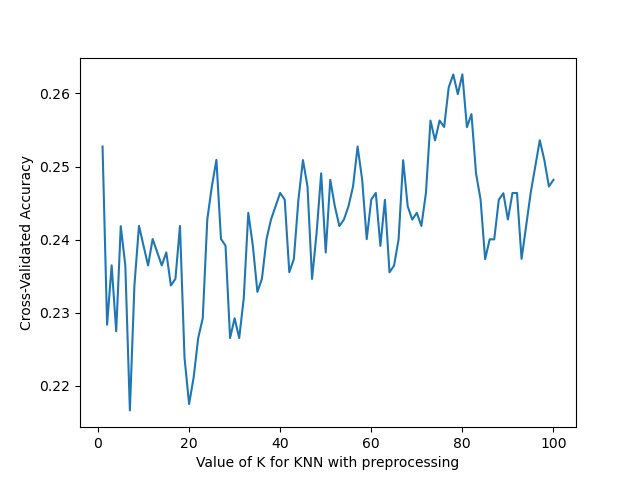
\includegraphics[width=0.55\columnwidth]{figures/K NeighBor Preproc.png}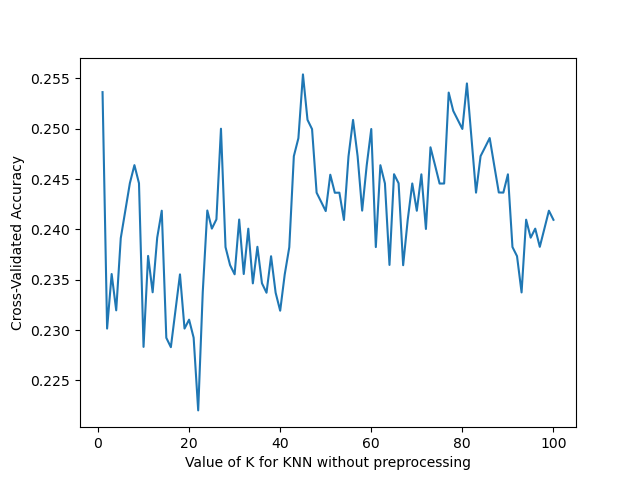
\includegraphics[width=0.55\columnwidth]{figures/K neight No Preproc.png}
    \caption{Cross Validation Accuracy al variare di K neighbor}
    \label{fig:target}
\end{figure}


\subsection{Ensemble}\label{ssec:Ensemble}

La tecnica di ensemble viene impiegata per combinare più modelli, detti \textbf{weak estimator}, per risolvere uno stesso problema. Vengono poi combinati per raggiungere un modello finale, \textbf{l'ensemble} per ottenere maggiori prestazioni. 
\newline Esistono diversi modi per effttuare l'ensemble, tra i quali:
\begin{itemize}
    \item \textbf{bagging}: si addestrano in parallelo n weak models e li si combina in ottica deterministica
    \item \textbf{boosting}: si addestrano in sequenza n modelli e li si concatena in maniera deterministica. Per cui ogni weak learner dipende dai precedenti.
    \item \textbf{stacking}: ogni modello viene considerato diverso (eterogeneità) e si addestra in parallelo in modo indipendente. Successivamente si combinano tutti i weak learner e si addestra il meta modello finale per effettuare predizioni sulla base dell'output designato dai weak learner.
\end{itemize}
L'ensemble, che è stato da me utilizzato, è tramite la tecnica di bagging, cioè un meta-stimatore di insieme che si adatta ai classificatori di base, ciascuno su sottoinsiemi casuali del set di dati originale e quindi aggrega le loro previsioni individuali (mediante voto o media) per formare una previsione finale. Ciò può inoltre ridurre la varianza dello stimatore base come il Decision Tree. Per questa ragione viene impiegato sui classificatori K-NearestNeighbor e Decision Tree che hanno più alto grado di accuracy.

\begin{figure}[H]
    \centering
    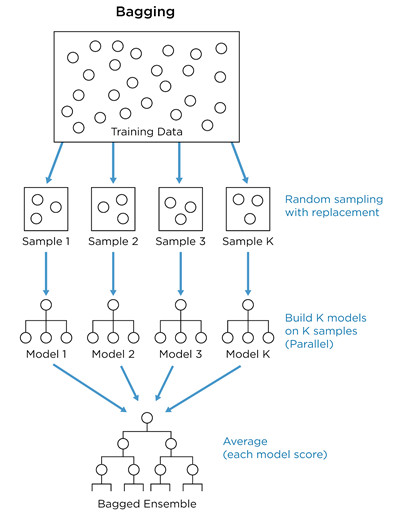
\includegraphics[width=0.35\columnwidth]{figures/Bagging_Ensemble.jpg}
    \caption{Bagging Ensemble}
    \label{fig:target}
\end{figure}